\documentclass[11pt]{article}

\usepackage[margin=.75in]{geometry}
\usepackage[T1]{fontenc}
\usepackage[utf8]{inputenc}
\usepackage{graphicx}

\setlength{\parindent}{0pt}
\setlength{\parskip}{0.6em}

\begin{document}

\title{Teensy Vibration Classifier}
\author{Charles Friley}
\date{December 2025}
\maketitle

\section{Motivation and Goal}
This project is a proof of concept, vibration-based object classification system. 
The goal is to show the end-to-end pipeline that detects an impact, captures vibrations, and then classifies the object using a trained neural network running on a microcontroller.

\section{System Concept}
A physical impact on a mounted plate is converted into a short accelerometer time series. 
That time series is passed through a trained neural network to classify the object dropped on the plate.
Everything is run locally on a Teensy 4.1 chip.

\section{Mechanical and Electrical Design}

\begin{figure}[ht]
  \centering
  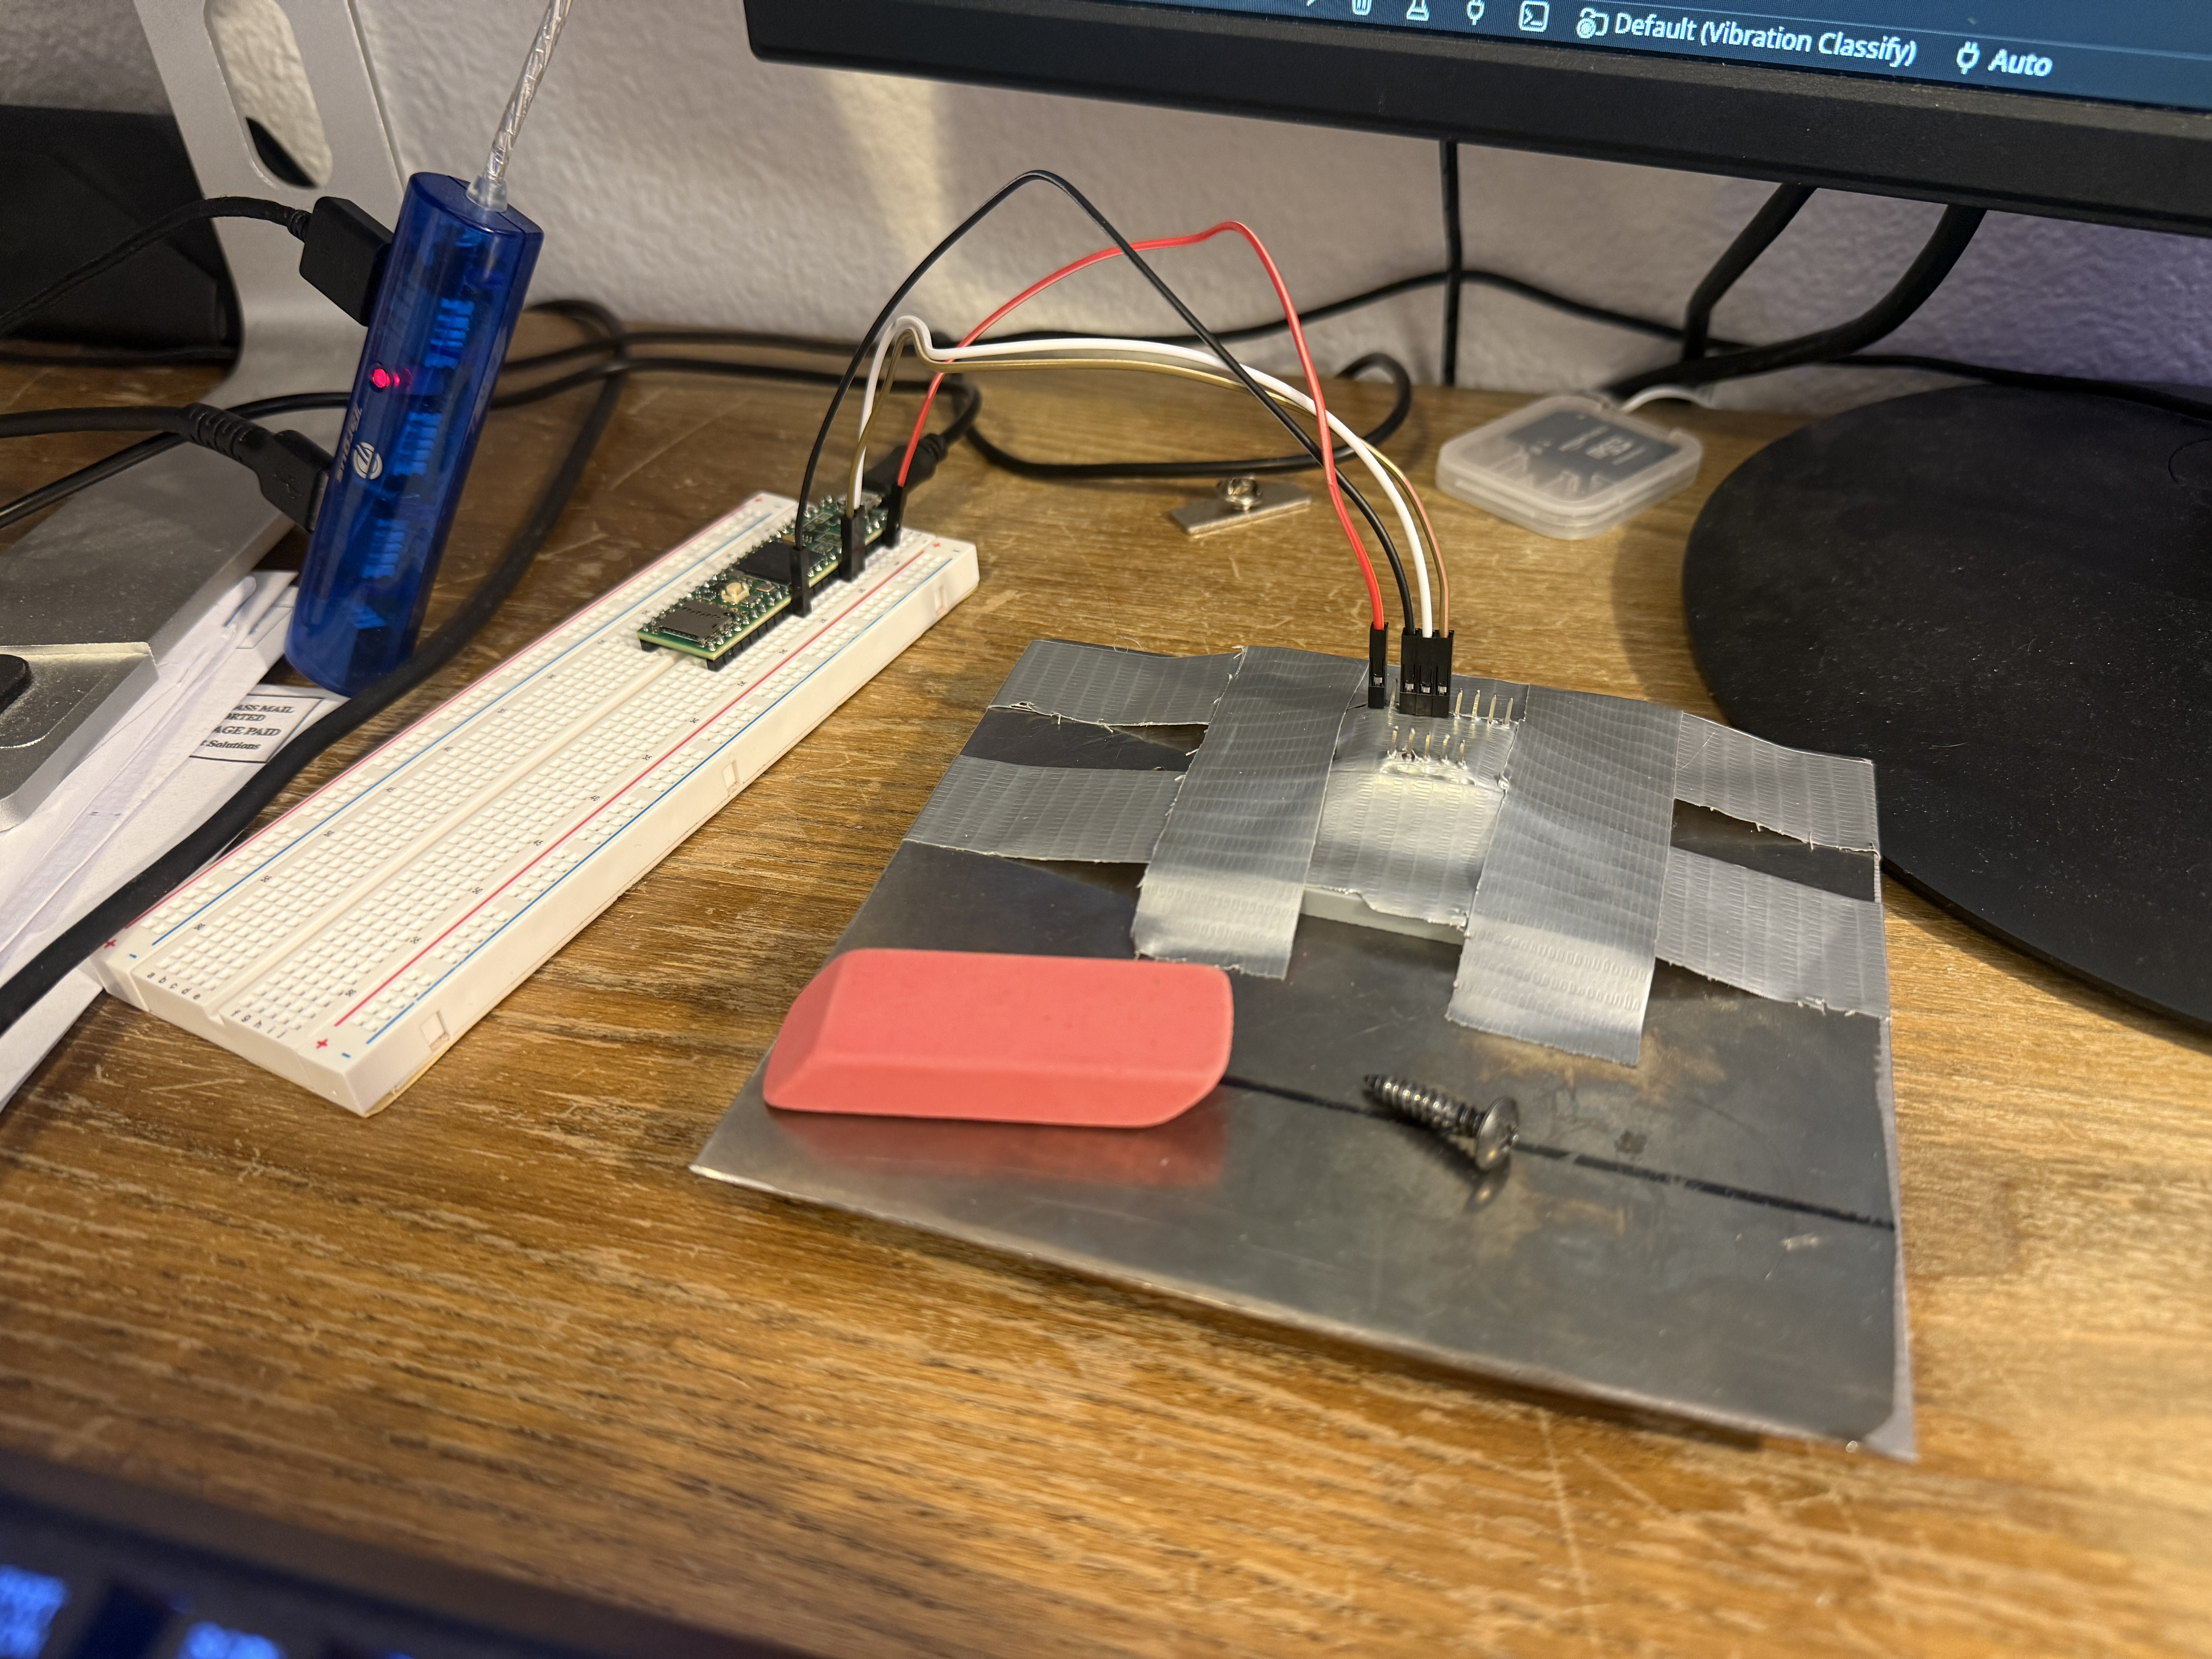
\includegraphics[width=0.7\linewidth]{figures/device.JPG}
  \caption{Vibration classifier hardware setup. A Teensy on a breadboard reads an IMU mounted rigidly to the steel plate. The two test objects used in the demo (eraser and screw) are shown resting on the plate. The TPU feet that support/isolate the plate are mounted underneath and are not visible in this photo.}
  \label{fig:device}
\end{figure}

As shown in figure~\ref{fig:device}, a thin steel plate is placed on top of 4 small 3D printed TPU legs with about 10\% infill. 
The feet isolate the plate from the table while allowing the plate to ring after impact.
An IMU is placed upside down in a 3D printed mount, and that mount is rigidly attached to the plate by duct tape.
The Teensy is off to the side and serial outputs are sent to the computer.

\section{Data Acquisition and Impact Triggering}
The firmware samples the accelerometer at 1660 Hz and uses a staged capture window after each impact. 
A small pretrigger buffer (128 samples) is always maintained so the recorded window includes the lead-in to the event. 
After the trigger fires, the firmware records 1024 full-rate samples, followed by a 1024-sample tail that is decimated by a factor of 4. 
This gives about 3.1 seconds of total coverage while keeping memory and compute bounded.

The firmware tracks a drifting baseline acceleration magnitude with an exponential moving average, then triggers when $|a|$ deviates far enough from that baseline. 
Hysteresis is used to re-arm the trigger only after the signal returns close to baseline, and a short refractory lockout prevents immediately re-triggering on the same event.

\section{Feature Extraction and Embedded Processing}
The magnitude of the acceleration is computed in order to reduce sensitivity to axis alignment and the orientation of the sensor. 
The peak magnitude provides a simple indicator of initial impact intensity. 
The RMS deviation from the baseline is computed over the full-rate stage (stage 1) to summarize overall vibration strength early in the response. 
A decay related feature captures how quick the vibration energy shrinks after impact. 

\subsection{Waveform Characteristics}
Figures~\ref{fig:eraser_waveform} and~\ref{fig:screw_waveform} show example acceleration-magnitude waveforms for a single eraser impact and a single screw impact.
Both signals exhibit a sharp impulse followed by resonant ringing of the plate, but the screw generally produces higher peak magnitudes and a faster decay.
These differences motivate the use of simple, embedded-friendly features. Rather than running a full FFT, the firmware also computes a small set of coarse narrow-band energies using Goertzel filters at 80/160/320/640 Hz.

\begin{figure}[ht]
  \centering
  \includegraphics[width=0.95\linewidth]{figures/impact_000061_label_eraser_side.png}
  \caption{Example acceleration-magnitude waveform for an eraser impact.
  The impact produces a moderate peak followed by a relatively long decay as the plate rings down.}
  \label{fig:eraser_waveform}
\end{figure}

\begin{figure}[ht]
  \centering
  \includegraphics[width=0.95\linewidth]{figures/impact_000141_label_screw.png}
  \caption{Example acceleration-magnitude waveform for a screw impact.
  The screw produces a sharper impulse with higher peak magnitude and faster decay compared to the eraser.}
  \label{fig:screw_waveform}
\end{figure}

\subsection{Repeatability Across Trials}
Figures~\ref{fig:stacked_eraser} and~\ref{fig:stacked_screw} show stacked acceleration-magnitude waveforms across many trials for the eraser and screw classes.
Within each class, the overall waveform shape is consistent despite small variations in peak timing and amplitude.
\begin{figure}[ht]
  \centering
  \includegraphics[width=0.95\linewidth]{figures/stacked_waveforms_eraser.png}
  \caption{Stacked acceleration-magnitude waveforms for multiple eraser impacts.
  The responses show consistent ringing behavior with relatively lower peak magnitudes and longer decay.}
  \label{fig:stacked_eraser}
\end{figure}

\begin{figure}[ht]
  \centering
  \includegraphics[width=0.95\linewidth]{figures/stacked_waveforms_screw.png}
  \caption{Stacked acceleration-magnitude waveforms for multiple screw impacts.
  Compared to the eraser, the screw impacts produce higher peak magnitudes and a faster decay envelope.}
  \label{fig:stacked_screw}
\end{figure}

\section{Model and On-Device Inference}
A small neural network is trained offline using labeled vibration windows collected on the device. 
The network takes the extracted features as input and outputs a class probability for each object type.
The model is kept small to meet memory and timing constraints in order to run locally on the microcontroller. 
The size of the neural network used in the demo was 8 inputs $\rightarrow$ 16 hidden units (ReLU) $\rightarrow$ 1 output logit (binary classification), with the same median imputer and standard-scaler preprocessing applied on-device.
The trained weights are embedded directly into the firmware, meaning that the weights are put into a large matrix in the \texttt{include/model\_weights.h} file. This is done automatically by a python script.
The classification results are streamed over Serial for demonstration, however in a proper implementation this system would route outputs to the rest of the sorting machine.


\section{Demonstration Evidence}
The photo in \texttt{figures/device.JPG} documents the physical layout of the plate, IMU mounting, and embedded electronics.\par
The video \texttt{figures/collecting\_data.MOV} shows labeled data collection by dropping a screw onto the plate while monitoring serial output.\par
The video \texttt{figures/predicting.MOV} shows real-time classification as an eraser and screw are dropped in random order.\par

\section{Results and Challenges}
This demonstration was able to correctly classify the two categories of objects the neural network was trained on, eraser and screws.
It achieved greater than 99\% accuracy under controlled test conditions.
The waveform consistency shown in Figures~\ref{fig:stacked_eraser} and~\ref{fig:stacked_screw} explains why a small neural network was sufficient for this task.
Classification is stable, but is less confident and accurate when the drop height or impact location varies significantly. 
This variability and limited training data are primary sources of classification error. 
Only 50 trials of the screw and 90 trials of the eraser were used to train.

\section{Limitations and Extensions}
The current system is limited to a small set of very different object classifications. This approach could be extended by collecting more data and expanding the neural network size and/or architecture.
A similar approach could be brought to a smartphone based implementation using the phone's IMU sensors and the much more powerful computer chips on the device for portable demonstration.

\section{Conclusion}
This project demonstrates a complete embedded sensing and inference pipeline running in real time on a microcontroller.
The results show that simple vibration features and a tiny neural network are sufficient for basic object classification tasks.

\end{document}
